\documentclass[11pt]{article}

\usepackage{acl}

\usepackage{times}
\usepackage{latexsym}
\usepackage[T1]{fontenc}
\usepackage[utf8]{inputenc}
\usepackage{microtype}
\usepackage{inconsolata}
\usepackage{graphicx}
\usepackage{amsmath}
\usepackage{booktabs}
\usepackage{hyperref}
\usepackage{enumitem}

\title{Stability by Design: Optimizing Prompt Properties in Small Language Models via Sensitivity Metrics\thanks{Code available at \url{https://github.com/yanivmu/NLP_Stability_by_Design}}}

\author{
Yaniv Mualem (ID: 209127612) \\
\texttt{yanivmualem@mail.tau.ac.il}
\And
Sharon Levy (ID: 315140152) \\
\texttt{sharon14@mail.tau.ac.il}
\AND
Eden Daya (ID: 315285759) \\
\texttt{edendaya@mail.tau.ac.il}
\And
Avner Fivelovich (ID: 314948811) \\
\texttt{Avnerf@mail.tau.ac.il}
\AND
\textmd{Moodle Group Number: 14}
}

\begin{document}
\maketitle

\begin{abstract}
Prompt wording can have a large effect on small language models, yet the effect is not always visible through task accuracy alone. We study prompt robustness through input sensitivity under semantic-preserving perturbations, and ask whether three prompt properties, metacognition, structure, and politeness, systematically affect model behavior. We evaluate an inference-only framework on CoLA \citep{warstadt2019neural}, QASC \citep{khot2020qasc}, and CSQA \citep{talmor2019commonsenseqa} using locally runnable models spanning encoder-decoder and decoder-only architectures, including both base and instruction-tuned variants. Our evaluation separates baseline task competence from sensitivity so that repeated wrong answers are not mistaken for useful stability. The final results show a strong interaction between prompt style, model capability, and task type. Structured prompting helps most clearly on CoLA, but can sharply reduce accuracy on multiple-choice tasks. Politeness is the safest intervention overall, while metacognitive prompting is the most unstable. These findings suggest that prompt robustness in small models should be evaluated jointly with task competence, parseability, and output behavior rather than through sensitivity alone.
\end{abstract}

\section{Introduction}

Small language models (SLMs) are increasingly attractive for practical NLP deployment because they are cheaper to run, easier to host locally, and more suitable for privacy-sensitive or resource-constrained settings than frontier-scale models. At the same time, these practical advantages come with a limitation: model behavior can depend strongly on how a task is phrased. In practice, small changes to a prompt, such as synonym substitutions, paraphrases, added conversational phrasing, or altered output formats, may change the model's output and, as a result, its measured task performance.

This matters both scientifically and practically. From a scientific perspective, prompt instability makes evaluation harder to interpret. If two prompts express the same task intent but lead to different outputs, then part of the observed performance may reflect wording choices rather than the model's actual ability. From a practical perspective, instability reduces reliability. In real applications, prompts are often reformulated by users, developers, or other components in a pipeline. Ideally, these reformulations should not cause large and unpredictable changes in model behavior. This concern is especially relevant for SLMs, where limited capacity and weaker instruction-following may amplify the effect of superficial prompt variation.

Sensitivity, however, is not meaningful on its own. A model that gives the same incorrect answer across all prompt variants may appear stable even though it is not robust in any useful sense. For this reason, prompt robustness should be studied together with baseline task competence. In this paper, we study prompt robustness in SLMs through the lens of \textbf{input sensitivity}, while also checking whether a model performs the underlying task well enough for sensitivity scores to be interpretable.

Following \citet{lu-etal-2024-prompts}, we define prompt sensitivity as the extent to which a model's output changes when the original prompt is replaced with lightly perturbed variants that preserve its meaning. We adapt this framework to small, locally runnable models and use a controlled perturbation pipeline that generates semantic-preserving variants through synonym replacement and paraphrasing. Our goal is not only to measure instability, but also to ask whether particular prompt properties systematically affect it.

We focus on three prompt properties inspired by prior work on prompt design \citep{long-etal-2025-makes}. The first is \textbf{metacognition}, implemented through self-check or self-verification cues. The second is \textbf{structure}, implemented through explicit output constraints, in our case a fixed JSON response format. The third is \textbf{politeness}, implemented through courteous conversational phrasing. These conditions are compared against a standard zero-shot control prompt.

\textbf{Research question:} Do certain prompt properties, metacognition, structure, and politeness, make language models more stable when inputs undergo semantic-preserving perturbations?

To answer this question, we use an inference-only evaluation framework. For each prompt style, we run the same model on the original prompt and on several semantic-preserving perturbations, and we measure sensitivity using the variation ratio,
\[
s = 1 - \frac{f_m}{N+1},
\]
where $f_m$ is the frequency of the modal output across the original prompt and its $N$ perturbed variants. In the main setting of our implementation, this metric is computed over raw decoded outputs after minimal normalization, while task accuracy is computed over parsed task labels. Lower values indicate greater consistency across perturbations. We evaluate this framework on three benchmarks with different task structures: CoLA, a binary grammatical acceptability task; QASC, an 8-way multiple-choice science question answering task; and CSQA, a 5-way multiple-choice commonsense reasoning task. We test a suite of locally runnable models that includes both encoder-decoder and decoder-only architectures, as well as base and instruction-tuned variants.

Our contributions are as follows:
\begin{itemize}
    \item We formulate prompt robustness in SLMs as a measurable sensitivity problem, while emphasizing that sensitivity is only interpretable when the model shows non-trivial baseline task competence.
    \item We adapt a sensitivity-based evaluation framework to small, locally runnable models using a controlled perturbation pipeline based on semantic-preserving synonym replacement and paraphrasing.
    \item We analyze how metacognition, structure, and politeness affect both sensitivity and task performance across three benchmark settings with different output spaces and difficulty profiles.
\end{itemize}

\section{Related Work}

Our work connects two lines of research: work on \textbf{prompt design and prompt attributes}, and work on \textbf{prompt sensitivity and input stability}.

The first line of work asks what makes a prompt effective. Recent research has moved beyond treating prompts as isolated heuristics and instead describes them in terms of reusable and interpretable attributes. In particular, \citet{long-etal-2025-makes} propose a taxonomy of prompt attributes that organizes prompt design choices into dimensions such as metacognitive guidance, structural constraints, and stylistic framing. This perspective is central to our study because it makes prompt design easier to analyze systematically rather than only through trial and error. We build directly on this view by selecting three attributes, metacognition, structure, and politeness, and operationalizing them in a controlled evaluation setup.

The second line of work studies prompt quality through robustness to input variation. \citet{lu-etal-2024-prompts} analyze prompts in terms of \textbf{input stability}, showing that prompts differ substantially in their sensitivity to minor perturbations and that higher sensitivity often accompanies worse downstream performance. This work motivates our study in two ways. First, it suggests that prompt evaluation should consider not only accuracy, but also whether outputs remain stable under semantically equivalent reformulations. Second, it provides a concrete sensitivity metric, variation ratio, that can serve as a diagnostic signal during prompt evaluation.

Our work builds on both lines of research, but it also differs from them in several important ways. Compared with prior work on prompt attributes, we are not only interested in whether a prompt improves average performance, but also in whether it changes robustness under controlled perturbations. Compared with prior work on sensitivity, we focus specifically on \textbf{small, locally runnable models}, including both base and instruction-tuned variants, where prompt sensitivity may interact strongly with limited instruction-following ability and with the model's underlying task competence. In this setting, low sensitivity is not always desirable if it simply reflects consistently wrong behavior. For this reason, our framework separates baseline task competence from sensitivity analysis by checking out-of-the-box accuracy before interpreting robustness scores.

The gap we address lies in the connection between \textbf{how prompts differ in form} and \textbf{how prompts differ in robustness}. Work on prompt attributes explains how prompts can vary in structure, intention, and style. Work on sensitivity shows that prompts can vary in stability under perturbation. What remains less explored is the relation between these two questions in small-model settings: which prompt properties make prompts more or less stable, when greater stability aligns with better task performance, and when stability can become a misleading signal. We address this gap by combining an attribute-based view of prompting with a sensitivity-based evaluation framework.

\section{Method}

\subsection{Task Definition}

We study prompt robustness as a conditional prediction problem under semantic-preserving reformulation. Let $x$ denote an input instance, let $y$ denote its gold label, and let $p$ denote a prompt style. A model receives a prompted version of the input, produces a prediction $\hat{y}$, and is then evaluated both on the original input and on lightly perturbed variants of that same input.

Our setting includes three task types. In QASC, the input is a multiple-choice science question with eight answer options, and the target output is a single answer letter from A to H. In CoLA, the input is a sentence and the target output is a binary grammaticality judgment, represented as Yes or No. In CSQA, the input is a multiple-choice commonsense question with five answer options, and the target output is a single answer letter from A to E. In all cases, the task content remains fixed across prompt styles; only the framing of the instruction changes.

\begin{table}[h]
\centering
\small
\resizebox{\columnwidth}{!}{%
\begin{tabular}{@{}llllll@{}}
\toprule
Dataset & Task Type & Domain & Split & Classes & Random \\ \midrule
CoLA & Binary Class. & Grammar & Val & 2 & 50.0\% \\
QASC & 8-way MC & Science & Val & 8 & 12.5\% \\
CSQA & 5-way MC & Commonsense & Val & 5 & 20.0\% \\ \bottomrule
\end{tabular}%
}
\caption{Statistics for the evaluation datasets.}
\label{tab:datasets}
\end{table}

For each instance, we compare four prompt styles. The \textbf{control} condition is a standard zero-shot instruction. The \textbf{metacognition} condition adds self-check and verification cues. The \textbf{structure} condition constrains the model to respond in a fixed JSON format that separates a brief explanation from a final answer field. The \textbf{politeness} condition adds courteous conversational phrasing. The goal is not to optimize prompts for a single benchmark, but to test whether these prompt properties change the stability of model predictions under controlled reformulations of the same underlying input.

\subsection{Approach}

Our framework is inference-only. We do not fine-tune any model parameters. Instead, we evaluate how the same pretrained model behaves when the same task is presented through different prompt styles and through semantic-preserving input perturbations. The overall evaluation flow is summarized in Algorithm~\ref{alg:pipeline}.

\begin{table*}[t]
\centering
\small
\begin{tabular}{lp{12cm}}
\toprule
\textbf{Style} & \textbf{Example Prompt (CoLA)} \\ \midrule
Control & Is this sentence grammatically correct? Answer Yes or No. \newline Sentence: "The problem perceives easily." \newline Answer: \\
Metacognition & Is this sentence grammatically correct? Answer Yes or No. Before answering, carefully check the grammar rules. Verify your answer is correct. \newline Sentence: "The problem perceives easily." \newline Think about it carefully, then answer: \\
Structure & Analyze whether the following sentence is grammatically correct. \newline Sentence: "The problem perceives easily." \newline You MUST respond with valid JSON in this exact format: \{"reasoning": "...", "final\_answer": "Yes or No"\} \\
Politeness & Hello! I would really appreciate your help with this. Could you please tell me if this sentence is grammatically correct? Please answer with Yes or No. \newline Sentence: "The problem perceives easily." \newline Thank you! Your answer: \\ \bottomrule
\end{tabular}
\caption{Examples of the four prompt styles applied to a single instance from the CoLA dataset.}
\label{tab:prompt-examples}
\end{table*}

\begin{figure}[h]
\begin{minipage}{\columnwidth}
\begin{small}
\begin{tabular}{p{0.95\columnwidth}}
\hline
\textbf{Algorithm 1:} Sensitivity Evaluation Pipeline \\ \hline
\textbf{Input:} Dataset $D$, Model $M$, Style $S$ \\
\textbf{1. OOTB Screening:} \\
\hspace{1em} Evaluate $M$ on $D$ using Control prompt. \\
\hspace{1em} \textbf{If} Accuracy $<$ Threshold: \textbf{Exit}. \\
\textbf{2. Perturbation:} \\
\hspace{1em} \textbf{For} each item $x \in D$: \\
\hspace{2em} Generate $N$ semantic variants $\{x'_1, ..., x'_N\}$. \\
\textbf{3. Inference:} \\
\hspace{1em} Collect responses $R = \{M(S, x), M(S, x'_1), ..., M(S, x'_N)\}$. \\
\textbf{4. Metric Calculation:} \\
\hspace{1em} Calculate Sensitivity $s = 1 - \frac{modal\_count(R)}{N+1}$. \\
\hspace{1em} Parse $R$ to calculate Accuracy $a$. \\ \hline
\end{tabular}
\end{small}
\caption{The sensitivity-based evaluation process.}
\label{alg:pipeline}
\end{minipage}
\end{figure}

For each model-dataset pair, we first run an out-of-the-box (OOTB) accuracy check using the control prompt.
 This step verifies that the model performs the task at a level that makes sensitivity analysis meaningful. Only after this screening step do we run the full sensitivity experiment.

In the main experiment, we sample input instances and evaluate each prompt style separately. For every sampled instance, we construct one original prompt and $N$ perturbed variants. The model is run on all $N+1$ versions. We then record both the raw decoded outputs and the parsed task-level answers. For QASC and CSQA, parsing extracts a single answer letter. For CoLA, parsing extracts a Yes or No judgment. In the structure condition, the parser reads the \texttt{final\_answer} field from the JSON output; in the other conditions, it extracts the relevant label from plain-text output.

We use two perturbation strategies. The default strategy is synonym-based perturbation. The input text is tokenized and part-of-speech tagged, and candidate replacement words are restricted to content words such as nouns, verbs, adjectives, and adverbs. Very short words, stopwords, question words, and answer labels are excluded. Candidate synonyms are taken from WordNet, with preference for the most common senses in order to reduce semantic drift. When synonym replacement cannot produce enough distinct variants, the pipeline uses lightweight fallback transformations such as minor article changes, filler prefixes, or punctuation variation.

The second strategy is paraphrasing. Here, a separate small model is used to rewrite the input while preserving its meaning. The paraphrase generator cycles through multiple rewrite instructions and uses stochastic decoding to produce diverse variants. Duplicate paraphrases are removed, and any shortfall is again completed by the synonym-based fallback. In both perturbation modes, the final goal is the same: produce multiple variants that change surface form while preserving task intent as much as possible.

For each instance and prompt style, we compute sensitivity using the variation ratio over the model's raw decoded outputs after minimal normalization. Following the methodology of \citet{lu-etal-2024-prompts}, we evaluate sensitivity on raw text to capture not only label flips but also instability in formatting, hedging, and output style, which are critical components of prompt robustness in small models. In parallel, we compute task accuracy over parsed task labels.
 This separation lets us distinguish instability in generation from correctness on the task, and avoids treating repeated wrong answers as meaningful robustness.

\section{Experimental Setup}

\subsection{Data}

We evaluate the framework on three benchmarks with different task structures.

The first is QASC, an 8-way multiple-choice science question answering benchmark. Each example contains a question and eight candidate answers. In early pilot experiments, including the dataset's supporting facts made the task too easy for stronger instruction-tuned models, producing near-ceiling behavior and leaving little room for meaningful sensitivity comparisons. For this reason, the reported setup uses QASC without fact injection. The model therefore sees the question and answer choices, but not the additional supporting facts. This makes the benchmark more suitable for studying whether prompt style changes both robustness and performance under a non-trivial level of difficulty.

The second benchmark is CoLA, a binary grammatical acceptability task. Each example consists of a single sentence, and the model must decide whether it is grammatically acceptable. CoLA complements the multiple-choice datasets in two useful ways. First, it has a much simpler output space. Second, it evaluates a different kind of linguistic competence, grammatical judgment rather than answer selection among explicit alternatives.

The third benchmark is CommonsenseQA (CSQA), a 5-way multiple-choice commonsense reasoning task. Each example contains a question and five candidate answers. We include CSQA because it extends the multiple-choice setting beyond QASC and tests whether prompt effects generalize to a different reasoning domain. Together, QASC and CSQA let us compare two multiple-choice tasks with different knowledge demands, while CoLA provides a contrasting binary setting.

All experiments use the validation split of each benchmark. The final reported results are aggregated over repeated runs across seeds and perturbation settings under the finalized evaluation setup.

\subsection{Models}

We evaluate a set of locally runnable models chosen to vary along two dimensions: architecture and instruction tuning. The model suite includes both encoder-decoder and decoder-only systems, as well as both base and instruction-tuned variants.

Our encoder-decoder models are Flan-T5-Base and Flan-T5-Large. These models are useful reference points because they are explicitly instruction-tuned and relatively strong on zero-shot text-to-text tasks. Our decoder-only base models are Pythia-410M and Llama-3.2-1B. These models let us examine whether prompt sensitivity behaves differently when instruction-following ability is limited. Our instruction-tuned decoder-only models are Llama-3.2-1B-Instruct and Phi-3-Mini-4K-Instruct. These provide a comparison point within the decoder-only family between base and instruction-tuned behavior.

All models are loaded directly from HuggingFace and evaluated without any parameter updates. For causal models, padding is set on the left and the end-of-sequence token is used as a padding token when necessary. For instruction-tuned chat models, the framework automatically applies the tokenizer's chat template before generation. This keeps model-specific formatting separate from the core evaluation loop and ensures that each model is used in a way that is consistent with its intended interface.

\subsection{Implementation Details}

Because our study focuses on prompt sensitivity rather than adaptation or fine-tuning, there is no training stage in the usual sense. All experiments are performed with frozen pretrained models and deterministic inference.

Generation is run with greedy decoding so that differences in output are driven by prompt and input changes rather than by sampling noise in the evaluated model itself. We utilized greedy decoding to isolate the impact of prompt wording from sampling noise, ensuring that measured sensitivity reflects structural rather than stochastic variance.
 The maximum number of generated tokens is task- and style-dependent. Plain answer formats use shorter generation limits, while structured prompts use longer budgets because the model must produce a valid JSON object. Metacognitive prompts on CoLA are also allowed longer outputs so that self-check instructions are not systematically truncated before the model reaches a final answer.

The implementation is designed for reproducibility. Random seeds are fixed across Python, NumPy, PyTorch, and the Transformers library. The framework uses three experiment seeds, 105, 2266, and 86379, and each run is fully determined by its seed and configuration. The perturbation pipeline also uses seed control at the level of individual examples so that the same configuration reproduces the same perturbation set across runs. Models are executed on the best available device, including CUDA, Apple MPS, or CPU, and half precision is used for selected decoder-only models when supported.

\section{Evaluation}

We evaluate each model-prompt combination along two axes: task performance and sensitivity.

The first metric is \textbf{OOTB accuracy}. Before running sensitivity experiments, we measure the model's accuracy on unperturbed inputs using the control prompt. This serves as a screening step. If a model performs at or near random guessing, then sensitivity is not informative, because the model may simply be repeating the same wrong answer. In the final implementation, OOTB accuracy is computed over all sampled items rather than only over successfully parsed responses, so unparseable outputs count as incorrect. We also track parse rate separately in order to distinguish low task accuracy from formatting or parsing failures. The screening thresholds are dataset-specific. For QASC, the random baseline is 12.5\% and the valid-signal threshold is 40\%. For CoLA, the random baseline is 50\% and the valid-signal threshold is 60\%. For CSQA, the random baseline is 20\% and the valid-signal threshold is 40\%.

The second metric is \textbf{variation ratio}, which measures the dispersion of outputs across the original input and its perturbations:
\[
s = 1 - \frac{f_m}{N+1},
\]
where $f_m$ is the frequency of the modal output across the original prompt and its $N$ perturbed variants. Lower values indicate greater consistency, while higher values indicate greater sensitivity to reformulation. In the main setting of our experiments, this score is computed over raw decoded outputs after minimal normalization rather than over parsed task labels. This design choice treats changes in generated form as part of prompt instability, which is especially relevant for structured prompts and for instruction-following settings where formatting itself is part of the response behavior. At the same time, we keep task accuracy separate and always compute it over parsed task labels.

In addition to average variation ratio, we report \textbf{style-specific accuracy} on the original, unperturbed inputs used in the main experiment. This lets us compare prompt styles not only in terms of stability, but also in terms of whether increased consistency coincides with better or worse task performance. Together, these metrics allow us to distinguish several cases: prompts that are both accurate and stable, prompts that are accurate but unstable, prompts that are stable only at the level of output format, and prompts that appear stable only because the model gives the same incorrect answer repeatedly.

\section{Results}

We report results obtained with the finalized evaluation pipeline described above. The values below summarize the final aggregated result pool.

\begin{table}[t]
\centering
\small
\setlength{\tabcolsep}{4pt}
\begin{tabular}{lccc}
\toprule
Model & CoLA & QASC & CSQA \\
\midrule
Phi-3-Mini & 77.0 & 74.0 & 69.0 \\
Flan-T5-Large & 62.0 & 62.0 & 80.0 \\
Flan-T5-Base & 30.7 & 42.0 & 74.0 \\
Llama-3.2-1B & 70.0 & 0.0 & 1.0 \\
Llama-3.2-1B-Instruct & 70.0 & 11.0 & 19.0 \\
Pythia-410M & 65.0 & 11.0 & 17.0 \\
\bottomrule
\end{tabular}
\caption{OOTB accuracy (\%) across all model-dataset pairs under the final evaluation setup.}
\label{tab:ootb}
\end{table}

Table~\ref{tab:ootb} shows that model capability varies sharply by task. Flan-T5-Large and Phi-3-Mini are the only models that perform solidly across all three datasets. Flan-T5-Base performs well on the multiple-choice tasks but fails on CoLA. The smaller base decoder-only models perform competitively on CoLA but collapse on QASC and CSQA, which confirms that low sensitivity on weak model-task pairs would be difficult to interpret as genuine robustness.

Because Flan-T5-Large performs strongly across all three benchmarks, we use it as the main cross-task comparison in Table~\ref{tab:main-results}. This model also exhibits both positive and negative prompt-style effects, which makes it the most informative single case for the paper's main argument.

\begin{table*}[t]
\centering
\small
\setlength{\tabcolsep}{5pt}
\begin{tabular}{lcccccc}
\toprule
& \multicolumn{2}{c}{CoLA} & \multicolumn{2}{c}{CSQA} & \multicolumn{2}{c}{QASC} \\
\cmidrule(lr){2-3}\cmidrule(lr){4-5}\cmidrule(lr){6-7}
Style & Acc. (\%) & VR & Acc. (\%) & VR & Acc. (\%) & VR \\
\midrule
Control & 63.7 & 0.1621 & 83.2 & 0.2242 & 62.2 & 0.2345 \\
Metacognition & 67.7 & 0.1693 & 59.9 & 0.7021 & 36.9 & 0.6529 \\
Structure & 70.3 & 0.1344 & 50.4 & 0.2237 & 22.1 & 0.1428 \\
Politeness & 69.9 & 0.1778 & 83.4 & 0.2170 & 62.2 & 0.2377 \\
\bottomrule
\end{tabular}
\caption{Prompt-style comparison for Flan-T5-Large across the three main benchmarks. Acc. is task accuracy; VR is average variation ratio. Values are aggregated over the final result pool.}
\label{tab:main-results}
\end{table*}

Table~\ref{tab:main-results} reveals a clear interaction between prompt style and task structure. On CoLA, all three non-control prompt styles improve accuracy, and \textbf{Structure} is the strongest overall condition. It reaches 70.3\% accuracy and the lowest variation ratio, 0.1344, improving on the control prompt on both axes. \textbf{Politeness} also improves accuracy substantially, reaching 69.9\%, but it does so with a somewhat higher variation ratio. \textbf{Metacognition} improves CoLA accuracy as well, but only slightly and with a small increase in sensitivity.

The two multiple-choice tasks show a very different pattern. On CSQA, the control and politeness prompts perform best, at 83.2\% and 83.4\% accuracy respectively, while metacognition and structure cause large accuracy drops. Metacognition is especially unstable, with a variation ratio of 0.7021. On QASC, the same pattern becomes even stronger. Control and politeness again perform best, both at 62.2\% accuracy, while metacognition and structure cause very large degradations. Structure reduces QASC accuracy to 22.1\%, even though it also reduces variation ratio relative to the control prompt. This is exactly the kind of misleading stability that motivated our setup: low variation ratio does not necessarily indicate useful robustness if accuracy collapses at the same time.

\begin{figure}[t]
\centering
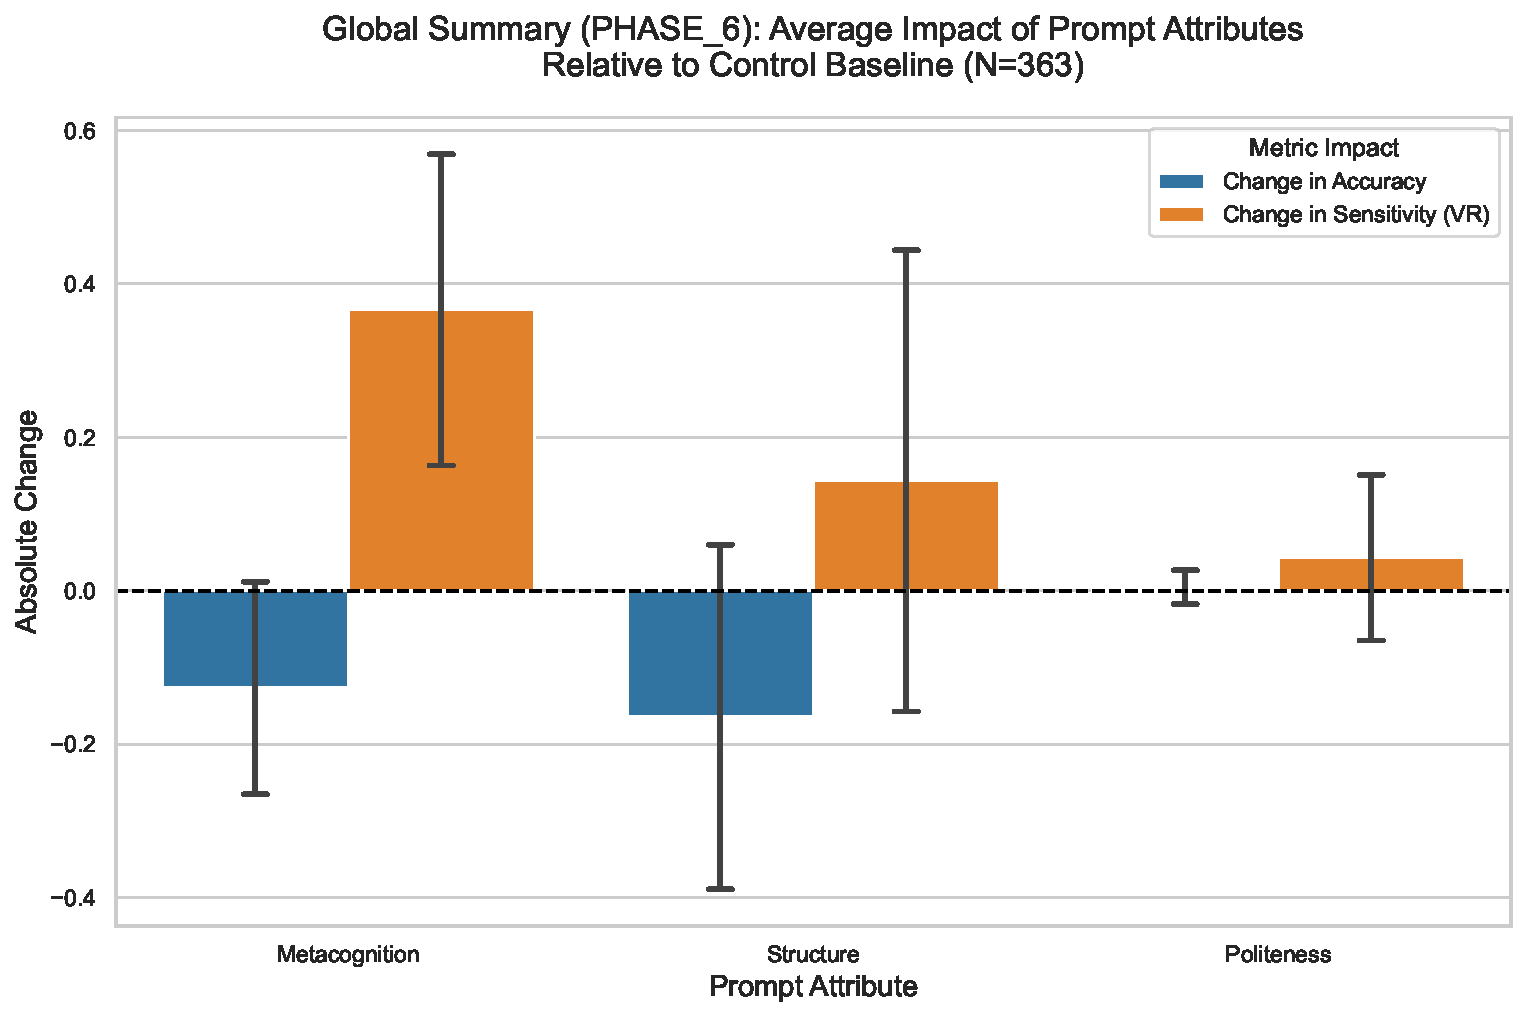
\includegraphics[width=\linewidth]{../outputs/figures/phase_6/summary_impact.pdf}
\caption{Impact of prompt attributes relative to the Control baseline across all tasks. Accuracy improvements are seen on CoLA, but structured prompting induces a significant trade-off on multiple-choice tasks.}
\label{fig:summary}
\end{figure}

Figure~\ref{fig:summary} visualizes the clearest positive result in our experiments. The CoLA setting shows that prompt design can improve both performance and robustness, but this effect is not general. The same styles that help on CoLA can harm performance sharply on CSQA and QASC.

\section{Discussion}

Across the full result set, three broader patterns emerge. First, \textbf{Politeness} is the safest prompt style. It is almost always neutral or slightly positive, and it never causes the kind of catastrophic failures seen with the other styles. Its strongest result appears on Flan-T5-Large for CoLA, where it improves accuracy by more than six percentage points.

Second, \textbf{Metacognition} is the riskiest style. It can help on a binary task such as CoLA for a capable instruction-tuned model, but it consistently harms performance on the multiple-choice tasks and often increases sensitivity sharply. The likely reason is that metacognitive prompts encourage longer, more verbose outputs, which makes answer extraction harder and increases the chance of derailment, especially in smaller or weaker models.

Third, \textbf{Structure} has mixed effects. On CoLA, structured JSON prompting can be genuinely helpful. On multiple-choice tasks, however, structure often produces the largest accuracy drops. In these cases, lower variation ratio may reflect rigid output behavior rather than robust reasoning.

Furthermore, we analyzed the computational load of different prompt styles. In our experiments with Phi-3-Mini on CSQA, the \textbf{Structure} prompt (which requires generating a JSON object with reasoning) increased average inference latency by approximately 14.6x compared to the Control prompt. This highlights a significant deployment trade-off: while structured outputs improve parsing reliability and can sometimes improve robustness, they introduce a heavy computational bottleneck, especially in decoder-only causal models where sequence length directly impacts generation time.

These results also suggest that task type matters.
 The binary CoLA setting tolerates prompt modifications better than the multiple-choice settings. By contrast, CSQA and QASC are both more brittle under prompt changes, and the negative effects are especially large when the prompt encourages extra reasoning or enforces a rigid output schema. Prompt robustness in small models therefore depends not only on the prompt itself, but also on the interaction between model capability and task structure.

\section{Limitations}

Our study has several limitations. First, the model suite is intentionally small and local, which is appropriate for the course project but limits generalization to larger frontier models. Second, although we evaluate three benchmarks, they still cover only a narrow slice of possible NLP behavior. All three are classification-style tasks, and the results may not transfer directly to more open-ended generation settings.

Third, our perturbation pipeline is controlled but imperfect. WordNet-based synonym replacement and model-based paraphrasing aim to preserve meaning, but neither method guarantees semantic equivalence in every case. Some perturbations may still change difficulty or emphasis in subtle ways. Fourth, the final reported results aggregate repeated runs across seeds and perturbation settings. This improves stability of the summary, but it also means that finer-grained differences between specific perturbation methods are not the focus of the main paper.

Finally, our primary sensitivity metric is computed over raw decoded outputs rather than parsed labels. This choice is defensible because output form is part of prompt behavior, but it also means that some measured instability reflects formatting differences rather than task-level answer flips. Comparing raw-output and parsed-label sensitivity more systematically would be a useful direction for future work.

\section{Conclusion}

We presented an inference-only framework for studying prompt robustness in small language models through sensitivity under semantic-preserving perturbations. Using prompt attributes drawn from prior work, metacognition, structure, and politeness, we examined how different kinds of prompt design affect both robustness and task performance on CoLA, QASC, and CSQA. Our findings support a cautious conclusion. Prompt properties do matter, but their effects depend strongly on model capability and task structure. CoLA provides the clearest case in which prompt design can help, while the multiple-choice tasks show that the same prompt changes can also harm performance substantially. For small models, robustness should therefore be evaluated jointly with accuracy, parseability, and output behavior rather than as a standalone property.

\section*{AI Usage Disclosure - UPDATE LATER}

We used AI tools (mainly GPT 5.4) for language editing, structural planning, and LaTeX drafting assistance. PLACEHOLDER

\bibliographystyle{acl_natbib}
\bibliography{custom}

\end{document}{acl_natbib}